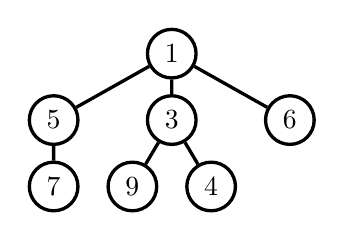
\begin{tikzpicture}[very thick, level/.style={sibling distance=15mm/#1}, level distance=24pt]

\node [circle, draw] (z){$1$}
child {
    node[circle, draw] (a) {$5$}
    child {
        node[circle, draw] (b) {$7$}
    }
}
child {
    node[circle, draw] (c) {$3$}
    child[sibling distance=10mm] {
        node[circle, draw] (d) {$9$}
    }
    child[sibling distance=10mm] {
        node[circle, draw] (e) {$4$}
    }
}
child {
    node[circle, draw] (f) {$6$}
};
\end{tikzpicture}
